\documentclass[preprint,5p]{elsarticle}
\usepackage{graphicx}
\usepackage{dcolumn}
\usepackage{bm}  
\usepackage{amssymb}  
\usepackage{hyperref}
\hypersetup{colorlinks=true, urlcolor=blue, citecolor=blue}
\usepackage[displaymath]{lineno}
\begin{document}

\title{\vspace{-15mm}\fontsize{24pt}{10pt}\selectfont\textbf{A Radial Time 
Projection Chamber for $\alpha$ detection in CLAS at JLab}}
\input author_list.tex  

\date{\today}

\begin{abstract}
A new Radial Time Projection Chamber (RTPC) was developed at the Jefferson 
Laboratory to track low-energy nuclear recoils for the purpose of measuring
exclusive nuclear reactions, such as coherent Deeply Virtual Compton Scattering
and coherent meson production off $^4$He. In such processes, the $^4$He nucleus
remains intact in the final state, however the CEBAF Large
Acceptance Spectrometer (CLAS) cannot track the low energy $\alpha$ particles. In
2009, we carried out measurements using the CLAS spectrometer supplemented by
the RTPC positioned directly around a gaseous $^4$He target, allowing a detection
threshold as low as 12~MeV for $^4$He. This article discusses the design,
principle of operation, calibration methods and the performances of this RTPC.
\end{abstract}

\maketitle

\section{Introduction} \label{sec:level1}

Until recently, the Thomas Jefferson National Accelerator Facility, in 
Newport News, Virginia, USA, has provided high power electron beams of 
up to 6 GeV energy and 100$\%$ duty factor to three experimental Halls (A, B, C) 
simultaneously. The CLAS spectrometer~\cite{CLASref}, located
in Hall-B, was based on a superconducting toroidal magnet and composed of 
several sub-detectors. Figure~\ref{fig:CLAS} shows a three dimensional 
representation of the baseline CLAS spectrometer:
\begin{itemize}
 \item Three regions of Drift Chambers (DC) for the tracking of charged 
       particles~\cite{DCref}.
 \item Superconducting toroidal magnet to bend the trajectories 
       of charged particles, thus allowing momentum measurement with the DC tracking information.
 \item Threshold Cherenkov Counters (CC) for electron identification at momenta 
       $<2.7$ GeV~\cite{CCref}.
 \item Scintillation Counters (SC) to identify charged hadrons by measuring their 
       time of flight~\cite{TOFref}.
 \item Electromagnetic Calorimeters (EC) for identification of electrons, 
       photons and neutrons~\cite{ECref}.
\end{itemize}

\begin{figure}[tbp]
\centering 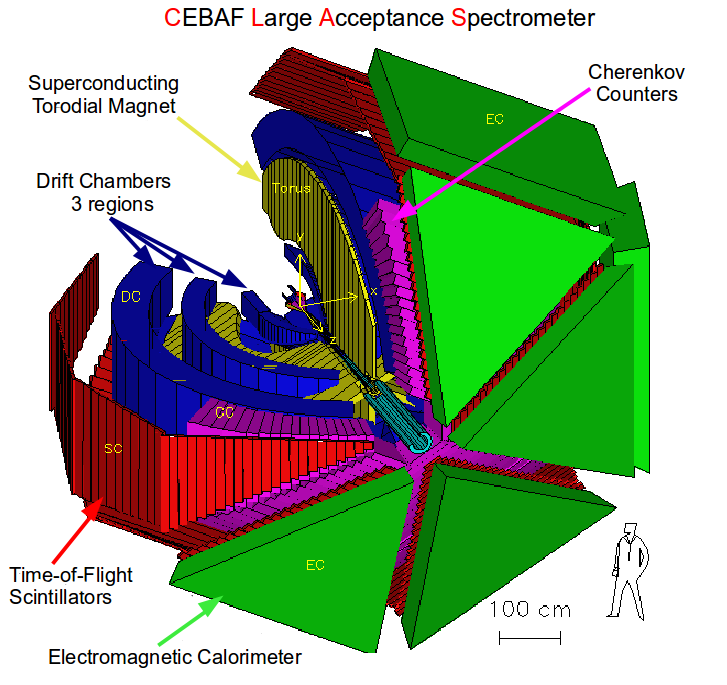
\includegraphics[scale=0.3]{fig/test_clas.png}
\caption{A three dimensional representation of the baseline CLAS setup. The
   full description is given in the text.} \label{fig:CLAS}
\end{figure}

For certain experiments the base CLAS system was complimented with ancillary 
detectors. For exemple, the measurement of the Deeply Virtual Compton 
Scattering (DVCS) process ($eH \rightarrow e' H' \gamma$, where $H$ is a 
nucleon or nuclei) necessitates an upgrade of the photon detection system. 
Indeed, with a 6 GeV electron beam, the majority of DVCS photons are produced 
at very forward angles, where the acceptance of the EC was poor. To extend the 
detection range, an inner calorimeter (IC) was built for the E01-113 
experiment in 2005~\cite{FX}. The IC is constructed from 424 lead-tungstate 
(PbWO$_{4}$) crystals, covering polar angles between 5$^{\circ}$ and 
15$^{\circ}$~\cite{Hyon-suk}. To protect the 
CLAS detector and the IC from the large flux of low energy M{\o}ller 
electrons, a 5~T solenoid was placed around the target to shield the detectors. 
To detect recoiling $\alpha$ particles from the coherent DVCS on helium, a new 
radial time projection chamber (RTPC) was developed to track low energy nuclear 
fragments. The solenoid field was used to track and measure momentum of 
particles in RTPC. The CLAS detector supplemented with IC and RTPC was used 
during a three months experimental run~\cite{proposal1,proposal2}
in 2009 with a longitudinally polarized electron beam of 130~nA 
and energy of 6.064 GeV incident on a gaseous $^{4}$He target.

The original design of the RTPC was developed for the BoNuS 
experiment at Jefferson Lab which took data with CLAS in 2005~\cite{BONUS-NIM}. An enhanced design, 
used in the 2009 DVCS experiment, is described in section \ref{sec_design} 
of this paper. Significant improvements were made to the RTPC mechanical 
structure and fabrication technique that both increased the acceptance and 
reduced the amount of material in the path of the outgoing particles. The 
data acquisition system described in section \ref{sec_readout} was reconfigured 
to increase the event readout rate. The calibration methods 
are discussed in section \ref{sec_calib}. The tracking algorithm is discussed in section
\ref{sec_tracking}. Finally, the overall performance
of the RTPC is described in section \ref{sec_perfor}.

\section{RTPC design} \label{sec_design}

With a 6 GeV incident electron energy, the recoiling $^{4}$He nuclei from coherent 
DVCS have an average momentum around 300 MeV/c (12 MeV kinetic energy). Such low energy $\alpha$ 
particles are stopped very rapidly, so the RTPC was designed to be as close 
as possible to the target and fit inside the 230~mm diameter bore of the 
5 Tesla solenoid magnet. 

\begin{figure}[tb]
\centering
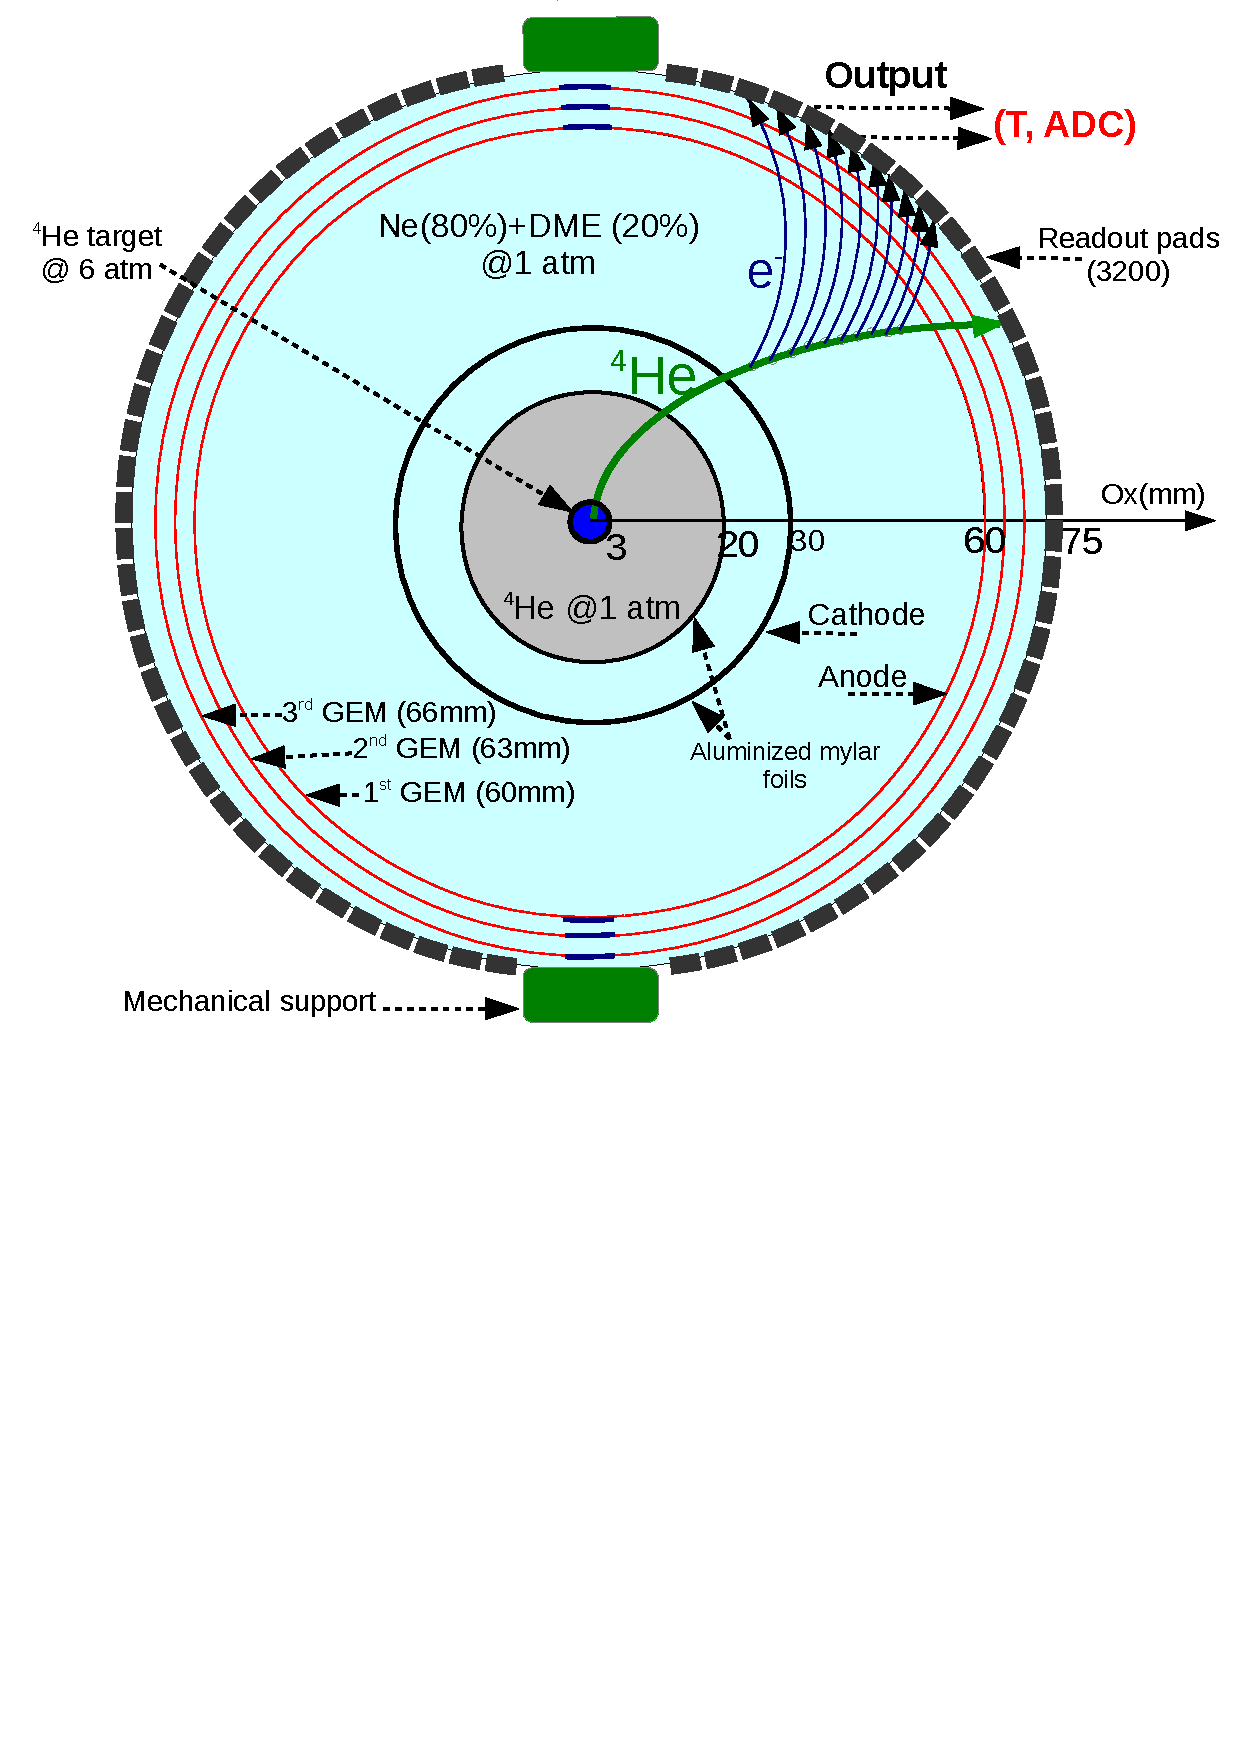
\includegraphics[{trim={0 12cm 0 0},clip, scale=0.4}]{fig_2017/RTPC_1_all.pdf}
\caption{Schematic drawing of CLAS RTPC in a plane perpendicular to the beam 
direction. See text for description of the elements.} \label{fig:RTPC_1_4}
\end{figure} 

The new CLAS RTPC is a 250~mm long cylinder of 158~mm diameter, leaving just enough 
room to fit pre-amplifiers between the RTPC outer shell and the solenoid. The 
electric field is directed perpendicularly to the beam direction, 
such that drifting electrons are pushed away from the beam line. These electrons 
are amplified by three layers of cylindrical gas electron multipliers (GEM) and 
detected by the readout system 
on the external shell of the detector as illustrated in the 
Fig.~\ref{fig:RTPC_1_4}. The RTPC is segmented into two halves with 
independent GEM amplification systems\footnote{The foils were produced by 
Tech-Etch, Inc.} that cover about 80\% of the azimuthal 
angle.

We detail here the different regions shown in Fig.~\ref{fig:RTPC_1_4} starting 
from the beam line towards larger radius:\\
\begin{itemize}
   \item The 6 atm helium-4 target extends along the beam axis; it 
      is a 284~mm long, 6~mm diameter straw with a 27-$\mu$m Kapton wall.
   \item The first gas gap covers the radial range from 3 mm to 20 mm. It is 
      filled with $^{4}$He gas at 1~atm to minimize secondary interactions from
      M\o{}ller electrons scattered by the beam. This region is surrounded by 
      a 4 $\mu$m thick window made of grounded aluminized Mylar.
   \item The second gap region extends between 20~mm and 30~mm and is filled with the 
      gas mixture of 80$\%$ neon (Ne) and 20$\%$ dimethyl ether (DME). This region 
      is surrounded by a 4~$\mu$m thick window made of aluminized Mylar set at $- 4260$~V 
      to serve as the cathode.
   \item The drift region is filled with the same Ne-DME gas mixture and extends 
      from the cathode to the first GEM, 60 mm away from the beam axis. The average 
      electric field in this region is perpendicular to the beam and about 550~V/cm.
   \item The electron amplification system is composed of three GEMs located at 
      radii of 60, 63 and 66 mm. In this configuration, the first GEM layer 
      serves as the anode and each subsequent GEM is set at a lower voltage to
      obtain a strong ($\sim$1600 V/cm) electric field between the GEM foils. A 
      275~V bias is applied across each GEM for amplification.
   \item The readout board has an internal radius of 69~mm and collects charge
     from the GEMs. Pre-amplifiers are plugged directly on its outer side and
     transmit the signal to the data acquisition electronics.
\end{itemize}

\begin{figure}[tbp]
\centering
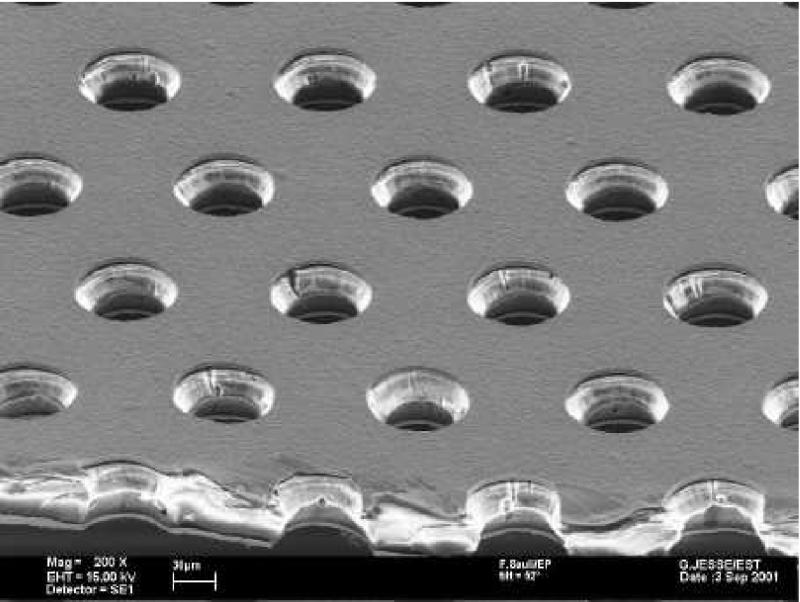
\includegraphics[scale=0.70]{fig/GEM_photo.jpg}
\caption{Image of a typical GEM foil similar to the one used for our RTPC 
\cite{GEM_ref_pic}.} 
   \label{fig:GEMs}
\end{figure}

The GEM technology has been chosen for the flexibility of the GEM foils,
which can be easily used to produce a curved amplification surface. Also, 
GEMs are known to have relatively low spark rate~\cite{GEM_ref}, which 
is important when trying to detect 
highly ionizing slow nuclei that deposit large amount of energy. The GEMs for 
this RTPC are made from a Kapton insulator layer, 300~$\mu$m 
thick, sandwiched between two 5~$\mu$m copper layers. The mesh of each GEM 
layer is chemically etched with 50~$\mu$m diameter holes with double-conical 
shapes as illustrated in Fig.~\ref{fig:GEMs}. The potential difference 
applied between the two copper layers of the GEM creates a very strong 
electric field in each hole leading to high ionization and amplification. 

The drift gas used in the experiment is a 80-20\% Ne-DME mixture. This choice 
has been made in order to balance the energy deposit, which is critical
for proper particle identification, with a reasonable
Lorentz angle. Calculations using the MAGBOLTZ program~\cite{MAGBOLTZ} 
showed that with the axial 5~T field, we would have a Lorentz angle of 
about 23$^\circ$ with this gas mixture.

One of the important challenge in developing the radial TPC was to obtain a 
good support structure for the GEM foils to allow a tractable 
installation of the GEMs. At the same time, we wanted to 
keep the material budget small in the forward region where we detect other 
particles in subsequent detectors. We successfully realized these prerequisites 
by using fiber glass rings glued to each end of the GEM foils to form self 
supporting cylinders that could be installed independently in the RTPC after 
gluing and soldering operations. The rigidity of the GEM foils was enough
for the structure to be self-supporting and only the upstream end of the cylinder 
was fixed to the main mechanical support structure. This design only left a 
light fiberglass ring in the downstream end, reducing to a minimum secondary 
interactions.

\section{Readout System} \label{sec_readout}

\begin{figure}[tb]
   \centering
   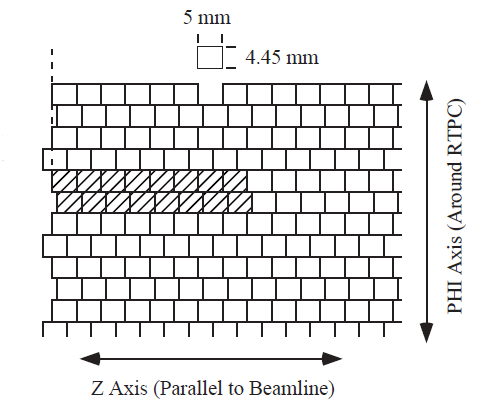
\includegraphics[scale=0.55]{fig/PADs.png}
   \caption[]{A schematic representation of a part of the readout system.  The 
   shaded sixteen pads are a group of pads that are connected to the same 
pre-amplifier.} \label{fig:PADs}
\end{figure}

The RTPC electron collection system has 3200 readout pads. These elements are
parallel to the GEMs, 69 mm from the central axis.
Figure~\ref{fig:PADs} shows a schematic drawing of the size and 
configuration of the pads. Each readout pad is 5 mm in length and 4.45 mm in 
width. The shift between the rows permits the reduction of aliasing. Each half of the 
RTPC has 40 rows and 40 columns of pads. The shaded region in Fig.~\ref{fig:PADs} 
shows how pads were grouped on 16 channel pre-amplifiers. The pre-amplifier boards, 
already employed in the BoNuS RTPC~\cite{BONUS-NIM}, serve the dual purpose of 
inverting the RTPC signals polarity -- from negative to positive -- to match the 
requirements of the subsequent readout system, and drive the 6~m long ribbon 
cable that connects to it.

\begin{figure*}[tb]
   \centering
   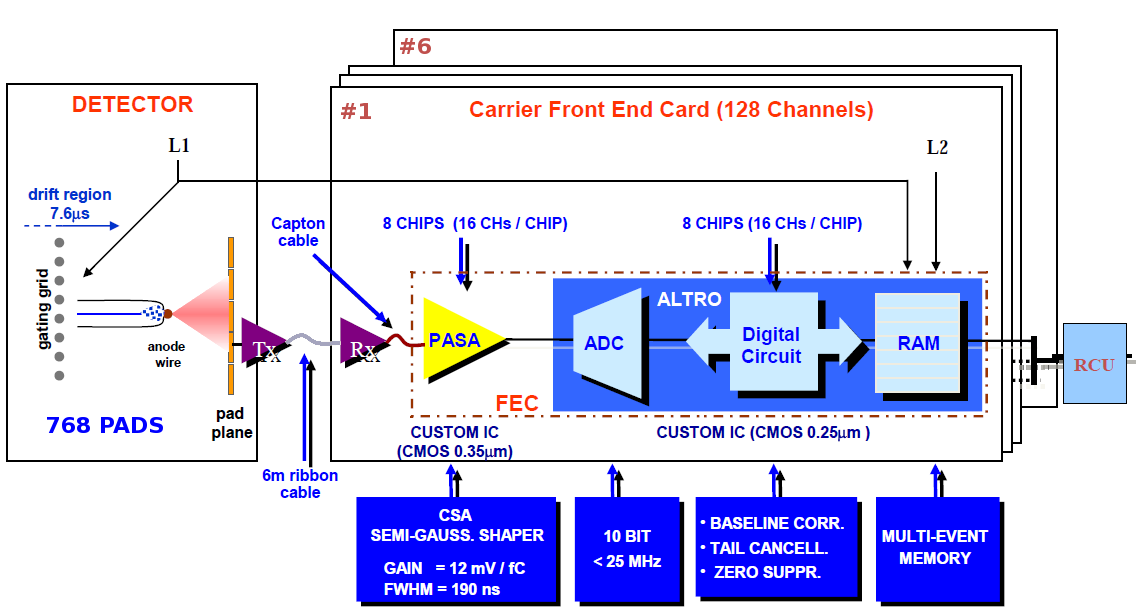
\includegraphics[width=.75\textwidth]{fig/ReadoutScheme.png}
   \caption[]{Schematic representation of the RTPC readout system, showing
   the different elements of the front end electronics.} 
   \label{fig:ReadoutScheme}
\end{figure*}

The readout system is based on the Front End Electronic (FEE) boards originally 
developed for the ALICE TPC readout system at CERN~\cite{ALICE-FEE}. Each 
readout channel is made of three main components: a charge sensitive, low 
impedance shaping amplifier, a 10 bit, 25-MHz digitizer, and a digital circuit 
that implements online-processing algorithms (pedestal subtraction, zero 
suppression, and tail cancellation). The amplifier is implemented in a 
fully-analogue ASIC, PASA~\cite{ALICE-PASA}, while the signal 
digitization and elaboration part is implemented in the digital ASIC, 
ALTRO~\cite{ALICE-ALTRO}. Both ASICs host 16 channels. The full readout 
chain is implemented on a single Front End Card (FEC), hosting 128 channels. 
FECs are hosted in custom crates, mounted close to the detector. A readout 
control unit (RCU) board is used to distribute the trigger signal to FECs 
and for data readout. Each RCU can handle up to 25 FECs with communication 
between them performed through a 
custom back-plane, implementing a low-voltage signal bus. The RCU communicates 
with the CLAS data acquisition (DAQ) system 
trough a 200 MB/s optical link, connected to a data acquisition PC hosting 
a ReadOut Receiver Card (RORC) used to interface with 
the CLAS DAQ system. An Ethernet link is also present, for slow-controls and 
monitoring.

The triggering and data-readout scheme is as follows. When a Level-1 (L1) trigger 
is received by a FEC-board, a programmable number of samples $N_0$ is digitized 
and stored in a data memory, and hence processed by the digital circuit. Upon 
arrival of Level-2 trigger, the latest processed samples are saved in a 
multi-event memory, individual to each-channel, ready for readout by the RCU.  
In our setup, the RCU receives the trigger signal from the CLAS Trigger 
Supervisor system, and distributes both L1 and L2 signals to all the FECs in 
the crate, with a definite L1-L2 trigger latency. Such latency is programmable, 
and has to be long enough to accommodate the digitization of the $N_0$ samples 
per channel.  In the current implementation, $N_0=100$ samples/channel are 
acquired for each trigger, operating ALTRO at the reduced sampling frequency of 
$10$~MHz. The L1-L2 latency is thus fixed to 15 $\mu$s.

The trigger signal also initiates RCU readout operation from FEC boards. All 
the measured samples from active channels are reported, together with a channel 
identifier and a time-stamp, to the RCU application, that in turns sends them 
on to the main event builder. During data reconstruction, the acquired samples are 
processed to obtain, for each readout pad, the accumulated charge (ADC) and the 
pulse time (T). Since pulse time was obtained as the time-stamp of the first 
sample above threshold, the resolution is equivalent to the ALTRO sampling 
time of 100~ns.

In order to reduce the data size, ALTRO is operated in zero-suppression mode: 
only samples above a programmable threshold are stored in the ALTRO on-board 
memory and then written to tape. A glitch-filter permits to reject spurious 
pulses due to noise, by requiring the presence of a minimum number of samples 
over threshold $N_{MINSEQ}$ to validate a sample. To properly reconstruct 
the signal shape, $N_{PRE}$ samples before threshold-crossing and $N_{POST}$ 
samples after the signal returns below threshold are saved. In the present 
configuration, $N_{MINSEQ}=N_{PRE}=N_{POST}=3$, while threshold is set just 
above the noise level. 

In order to read all the detector readout pads, four FEC crates are used, 
each equipped with 6 boards, plus a RCU. A schematic of the readout system, 
for a single crate, is reported in Fig.~\ref{fig:ReadoutScheme}. This 
configuration permits to reduce the dead time associated to FEC readout 
operations and to scale linearly with the number of boards in the crate. During the 
2009 run, the system was successfully operated with a DAQ rate of 3.1 kHz, with 
a live time of $70 \%$.

\section{Calibration} \label{sec_calib}

The timing information collected for each signal above threshold
is used to infer the origin of the ionization electrons and 
then the trajectory of the detected particle. Going from a collection of 
times to a momentum measurement based on the curvature of a track 
requires a good knowledge of the drift speed 
and drift paths followed by the electrons released in the gas. The recorded ADCs give 
the deposited energy per unit of length ($\small{\frac{dE}{dX}}$) which, 
together with the momentum calculated from the trajectory, enable the particle 
identification.

In this section we will detail the methods used to calibrate the drift speed,
drift paths and gains of the detector. Drift speed and paths were initially
calculated using the MAGBOLTZ~\cite{MAGBOLTZ} program, then refined using
data to account for variations of the run conditions. We always assume 
cylindrical symmetry in the chamber for the calibration, such that none of
the parameters depend on the azimuthal angle $\phi$. The initial MAGBOLTZ
calibration was improved through several iterations of the
process described below, with each time an increasing number of events 
properly reconstructed in the RTPC. The figures presented in this section
are the ones obtained while performing the last iteration of this
calibration process.

\subsection{Drift Speed Parametrization}

After the ionization, the released electrons 
drift to the cylindrical detection plane under the effect of the electric field. The 
electrons released close to the cathode take the most time to reach the readout 
pads, the cylindrical symmetry insures that the maximum distance is the same for all 
tracks. We illustrate this in Fig.~\ref{fig:RTPC_signals}, where we depict a 
typical $^{4}$He track. By measuring the maximum time ($T_{Max}$), we can infer the drift 
speed of the electrons in the RTPC.\\

\begin{figure}[tb]
\centering
%\includegraphics[scale=0.4][trim={0 5cm 0 0},clip]{fig_2017/RTPC_1_4.pdf}
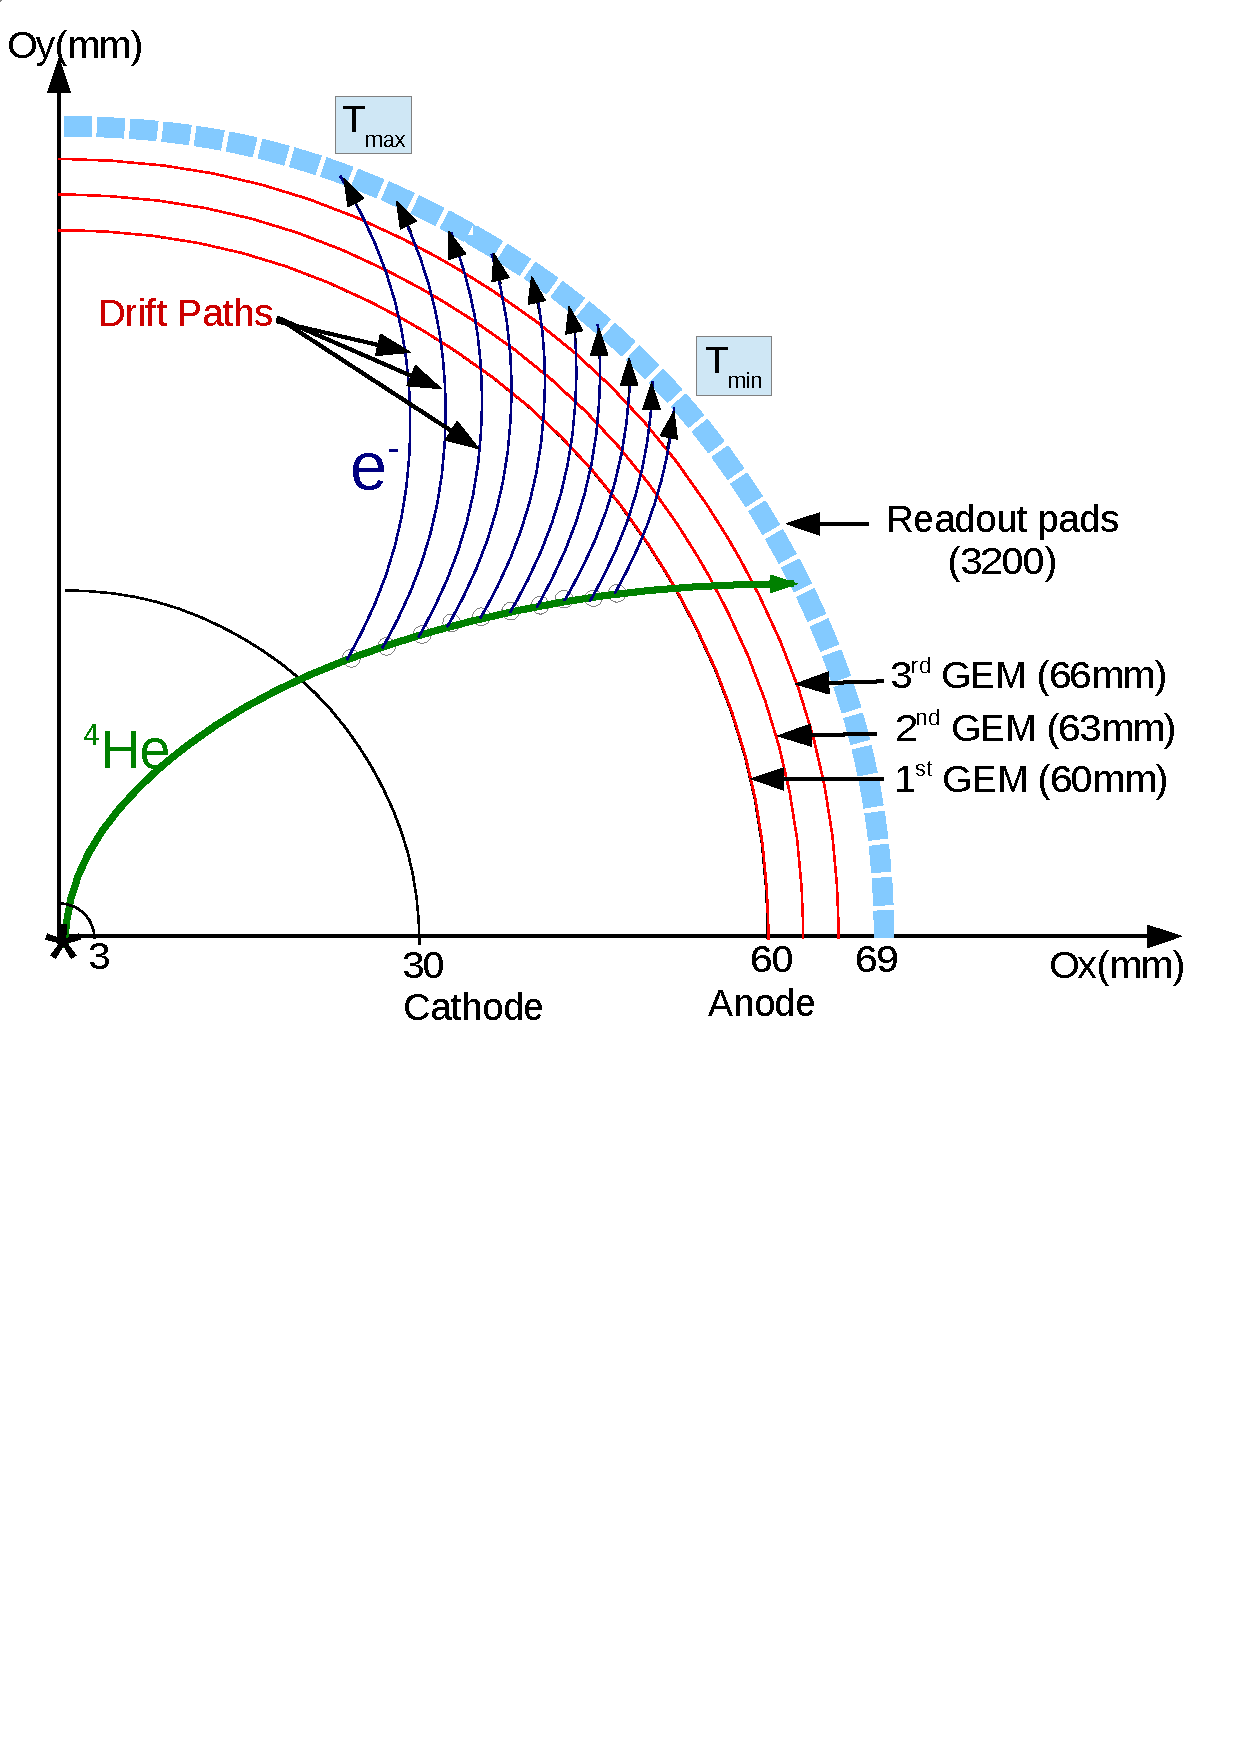
\includegraphics[{trim={0 12cm 0 0},clip, scale=0.4}]{fig_2017/RTPC_1_4.pdf}
\caption[]{A schematic drawing of a $^{4}$He track (in green) traversing the 
drift region, with the drift paths followed by the electrons (in black). } 
\label{fig:RTPC_signals}
\end{figure}

To measure the drift speed, we use the time profile of all hits in the 
chamber shown in Fig.~\ref{fig:TDC_profile}. We can clearly observe the 
dropping edge expected from geometrical considerations. We define a value $T_{Max/2}$ at 
which the dropping edge passes half the maximum number of hits in the 
histogram. This value was measured in bins along the 200~mm RTPC's length to take into 
account variations in the electric and magnetic field in the RTPC (see 
Fig.~\ref{fig:RunNumber_61551_TDCmax_Zslice}). 

\begin{figure}[tb]
   \centering
   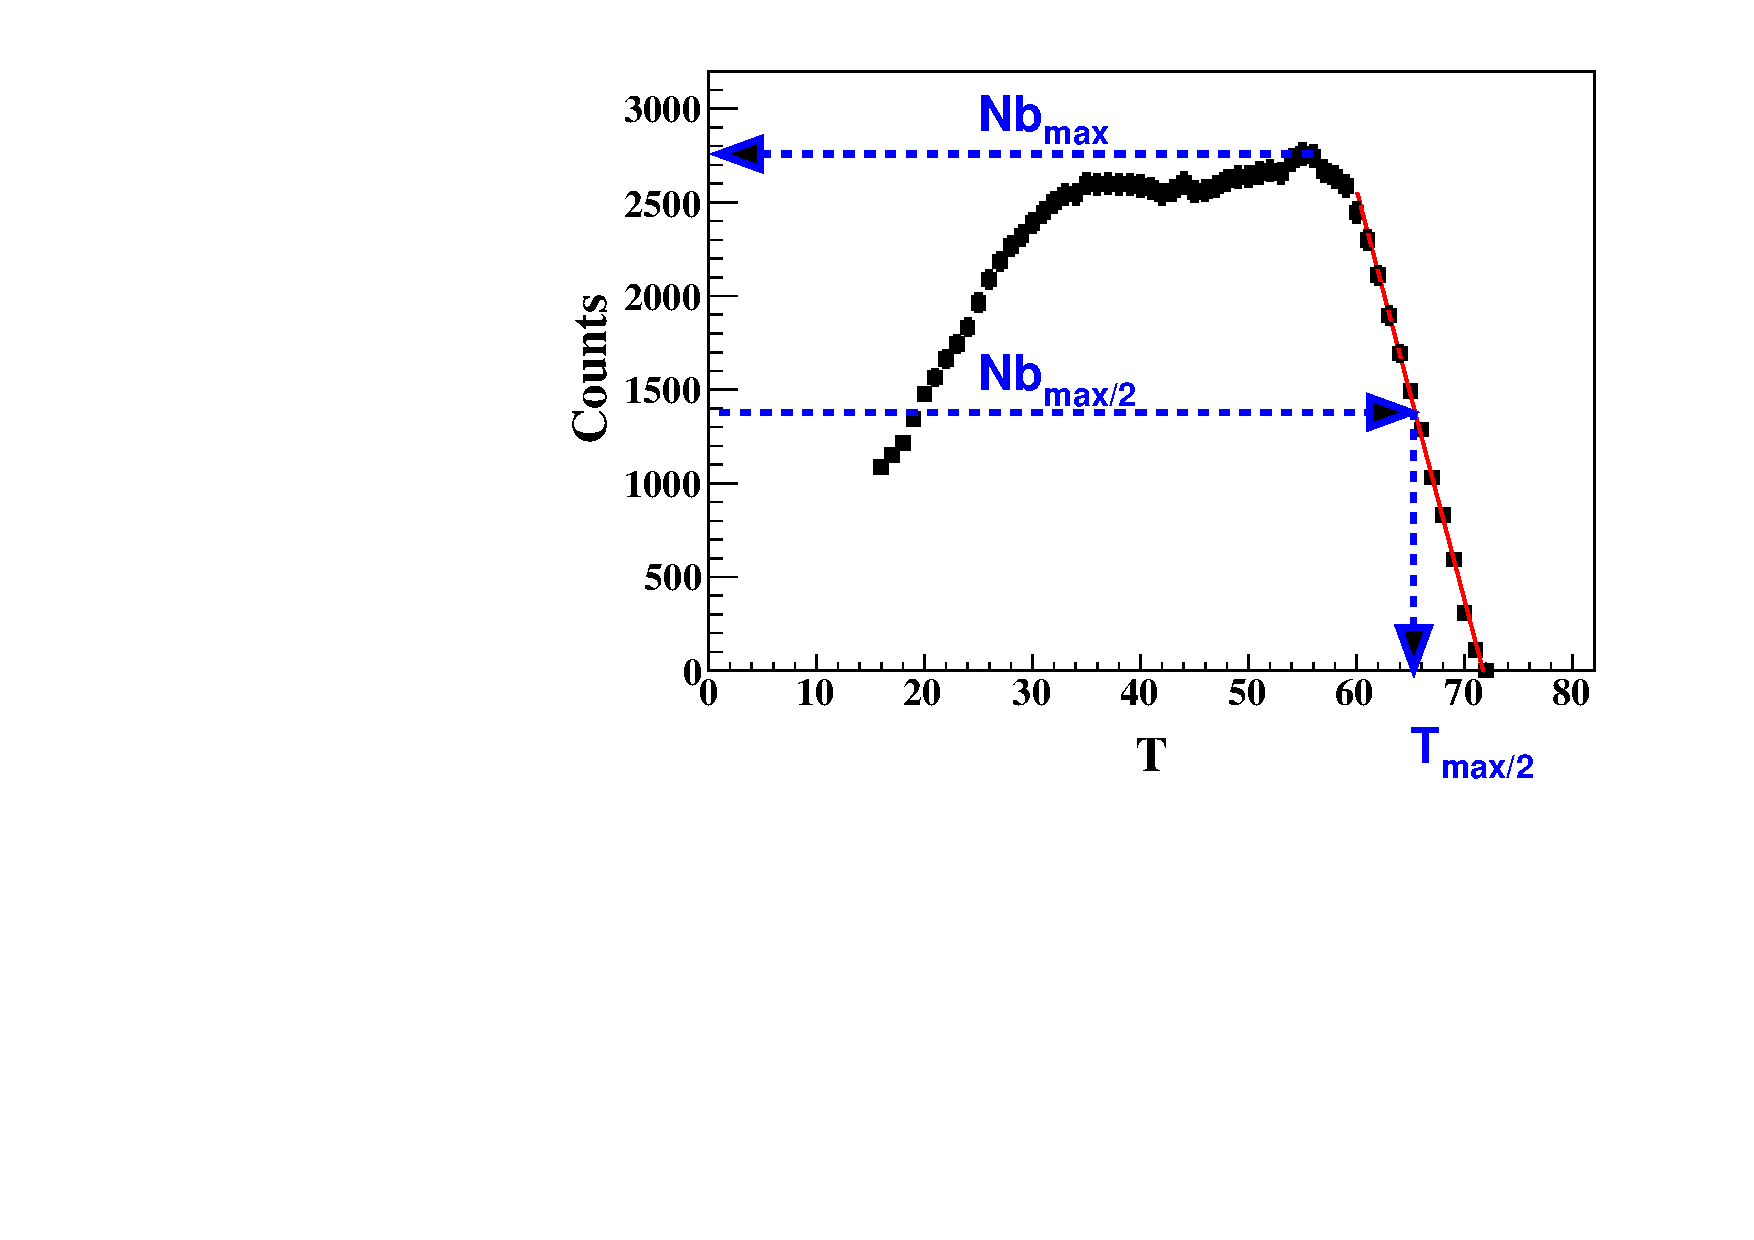
\includegraphics[scale=0.42]{fig_2017/hits_time_profile.pdf}
   \caption[]{Time distribution of the collected hits in one experimental run. Trigger
              time is defined as T=15, the time unit is the ALTRO sampling time of 100~ns.} 
   \label{fig:TDC_profile}
\end{figure}

\begin{figure}[tb]
\centering
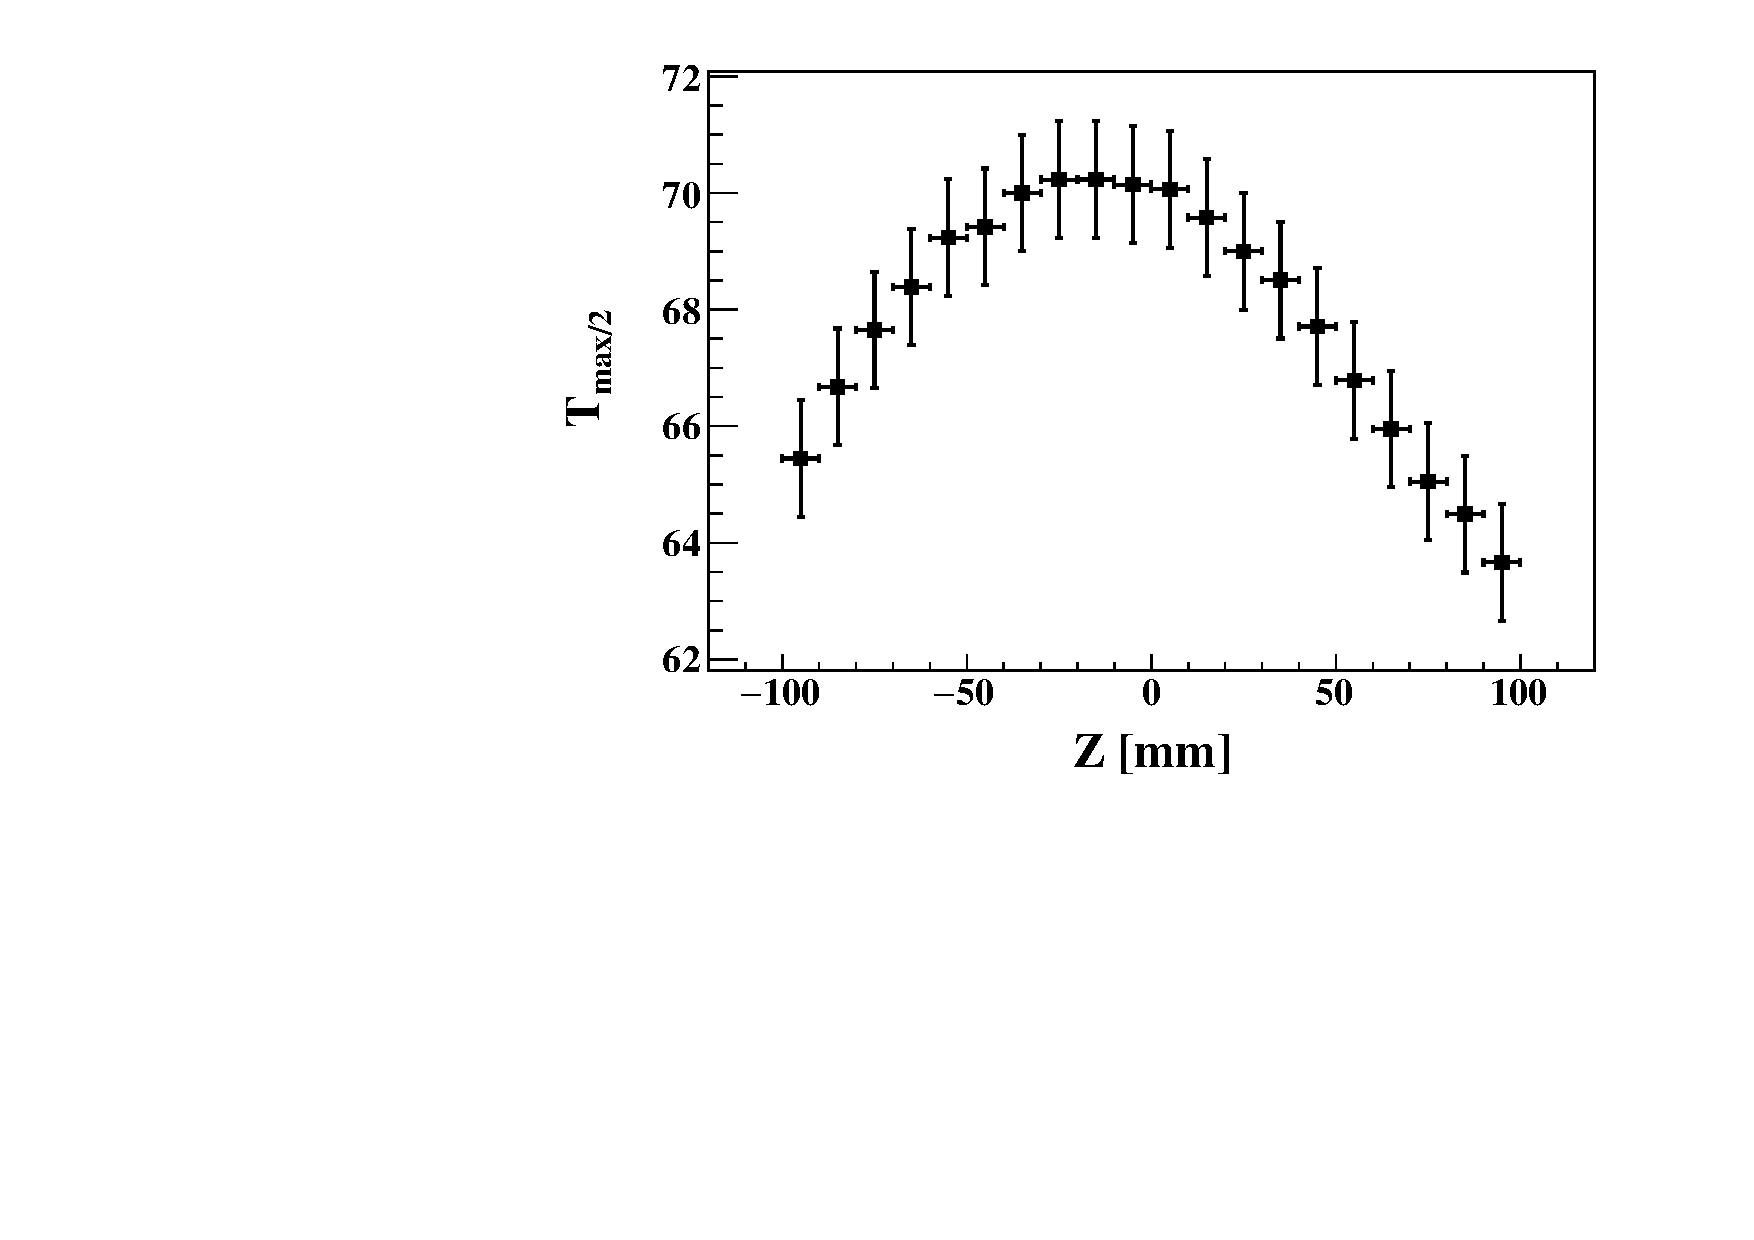
\includegraphics[scale=0.42]{fig_2017/RunNumber_61452_TDCmax_Zslice.pdf}
\caption{Maximum time of collected hits as a function of the track
              position on the $z$-axis for one experimental run. } 
\label{fig:RunNumber_61551_TDCmax_Zslice}
\end{figure}

Due to the non perfect experimental conditions, in particular possible contamination 
of our gas mixture, the drift speed changed during the three months long experimental 
run\footnote{We had to increase the gas flow during the experiment due to a small leak 
in the RTPC, which concurred to the large shift of drift time observed around run number 
61600. While our gas system was kept slightly over 
atmospheric pressure to avoid contamination from air or other external gases, it 
is likely that this leak was the source of modification of the gas mixture.}.  
Figure~\ref{fig:Drift_run_number_1} shows the $T_{Max/2}$ values for 
individual runs (approximately 2 hours long). We observe significant change in 
the drift speed before and after run 61600, while variations within these periods 
are ~2\%. These variations of the drift speed were accounted in the track reconstruction

\begin{figure*}[tb]
\centering
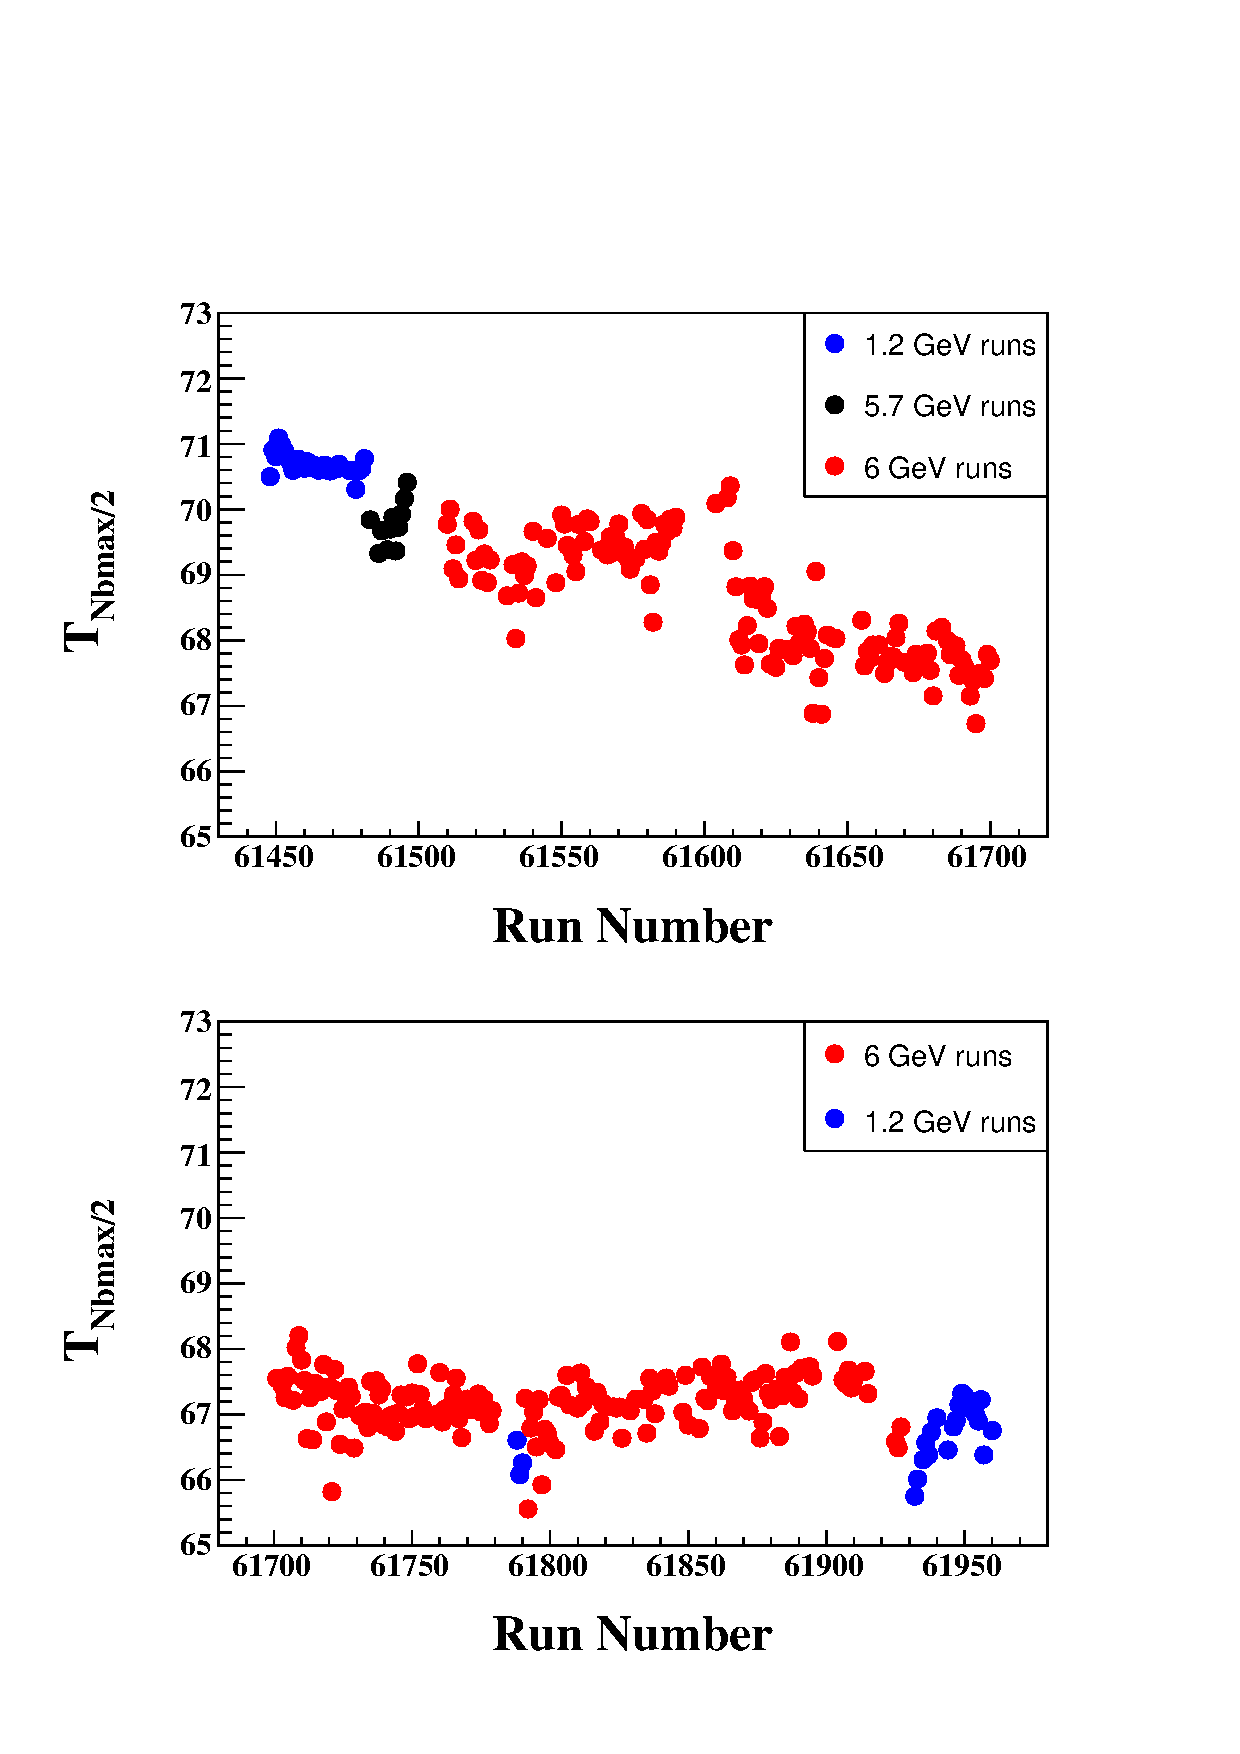
\includegraphics[width=16.5cm]{fig_2017/Drift_run_number.pdf}
\caption{$T_{max/2}$ versus the experimental run numbers.} 
\label{fig:Drift_run_number_1}
\end{figure*}


In summary, we obtain from our calibration a parame\-tri\-zation of the drift speed 
as a function of both position along the beam axis and the run number. These 
functions were extracted for our entire data set and implemented in the 
track reconstructions code.
   
\subsection{Drift Paths Calibration}

The drift path is the trajectory followed by the electrons released through 
ionization in the gas. We calculate them with
MAGBOLTZ~\cite{MAGBOLTZ}, but it requires knowledge of the detector's 
geometry, gas mixture composition, and of course the electric and magnetic 
fields over the whole volume of the detector. We used such calculation as a 
first calibration, but, 
as can be seen with the drift speed, conditions in the chamber were changing 
over time. Moreover, the 4 $\mu$m foil used as a cathode is easily deformed, such
that we expect the geometry accuracy to be of few millimeters, directly impacting 
our knowledge of the electric field. These problems, already 
encountered for the BoNuS RTPC calibration~\cite{BONUS-NIM}, motivated the 
acquisition of specific calibration runs. These were taken with a lower energy 
electron beam (1.204 and 1.269 GeV) to enhance the cross section of the elastic 
scattering ($e^{4}$He$\rightarrow e^{4}$He). In this process, the measurement of
the electron kinematics allows to calculate directly the kinematics of the Helium nucleus. 
By comparing the calculated momentum and angle of the recoil alpha particle to the 
measurement in the RTPC, we tuned the drift paths independently of our 
knowledge of the chamber's conditions.

Based on the kinematics of the electrons in the calibration data, 
we generate the helium nucleus in our RTPC GEANT4 simulation~\cite{GEANT4}. Then 
we compare the calculated GEANT4 trajectory of the Helium nuclei to 
the hits measured in the chamber. 
Because of the magnetic field, the drift paths are not linear in the RTPC. So 
to perform the extraction, we make a first approximation with a linear 
dependence between the radius of emission and the time of detection, and then 
refine our result. As it happens, the curvature is minimal and this process 
converges already on the second iteration. 

At the end of the extraction procedure, the azimuthal difference between the detection pad and 
the ionization point ($\Delta\phi$) is extracted as a function of time. 
In Fig.~\ref{fig:DELTA_PHI_TDC}, we show the resulting data points for one 
bin, where the drift path is easily identified and eventually fitted for 
implementation in our reconstruction codes.

\begin{figure}[tb]
\centering
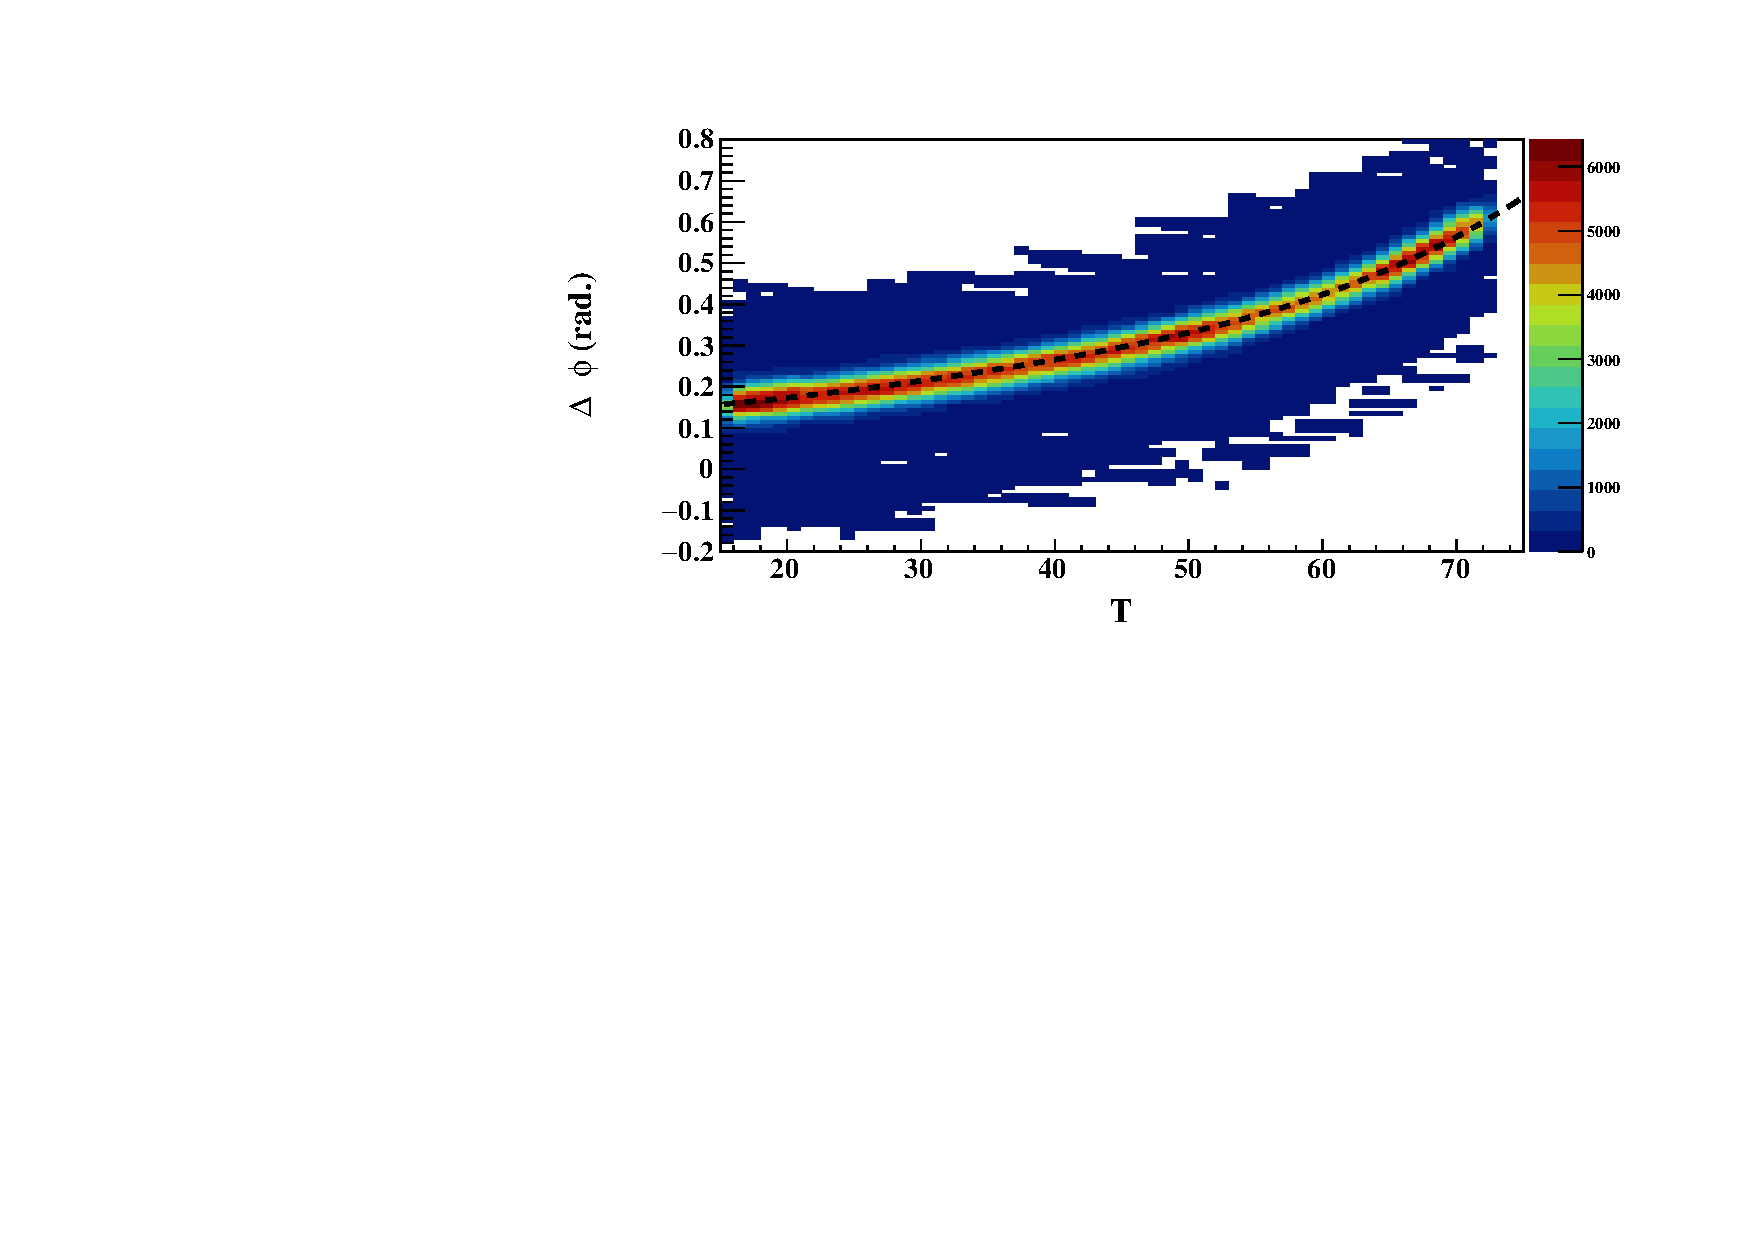
\includegraphics[scale=0.42]{fig_2017/FitResult_p2_11.pdf}
\caption{$\Delta \phi$ versus T distribution in the second pass for tracks
near 35 mm longitudinal position along the RTPC. The black line represents 
the final drift paths in this slice.}
\label{fig:DELTA_PHI_TDC}
\end{figure}

To verify the stability of the drift paths, this procedure was carried out 
using both the 1.204 GeV data from the beginning of the run period and the 
1.269 GeV data from the end of the run period (shown in blue on 
Fig.~\ref{fig:Drift_run_number_1}). Interestingly, we found very similar drift paths
for the two data sets and concluded that any changes in the system only
significantly affected the drift speed.

\subsection{Gain Calibration}

To calibrate the gains, we compare the experimental ADCs to the energy deposited 
for each pad individually in GEANT4 by similar simulated tracks (using the 
same elastic events as for the drift 
paths calibration). This requires a very good GEANT4 simulation 
including drift paths, but also the spread of the charge along the path
before reaching the pad, so that the simulated hits match the experimental 
ones. Moreover, the simulation has to match the DAQ features 
that can lead to cutting out hits. After setting the simulation properly, we 
compared simulation to experiment on an event by event basis as shown in 
Fig.~\ref{fig:EVENT_adc_tdc}. The gain for each pad is calculated 
as the ratio of the measured ADCs to the simulated deposited energy.  
Then, these gains are refined using correction factors obtained from a 
sample of good tracks. For each track, we calculate the corrected 
energy deposit on a pad and compare it to the average
deposit recorded by the other pads. This last step was implemented to 
avoid any bias from this simulation based calibration method.
Final results are shown in Fig.~\ref{fig:dedx_p_exp_2nd}, where energy 
loss of particles is plotted against momentum over charge ratio. One can 
clearly see the band for $^4$He in its expected position.

\begin{figure}[tb!]
   \centering
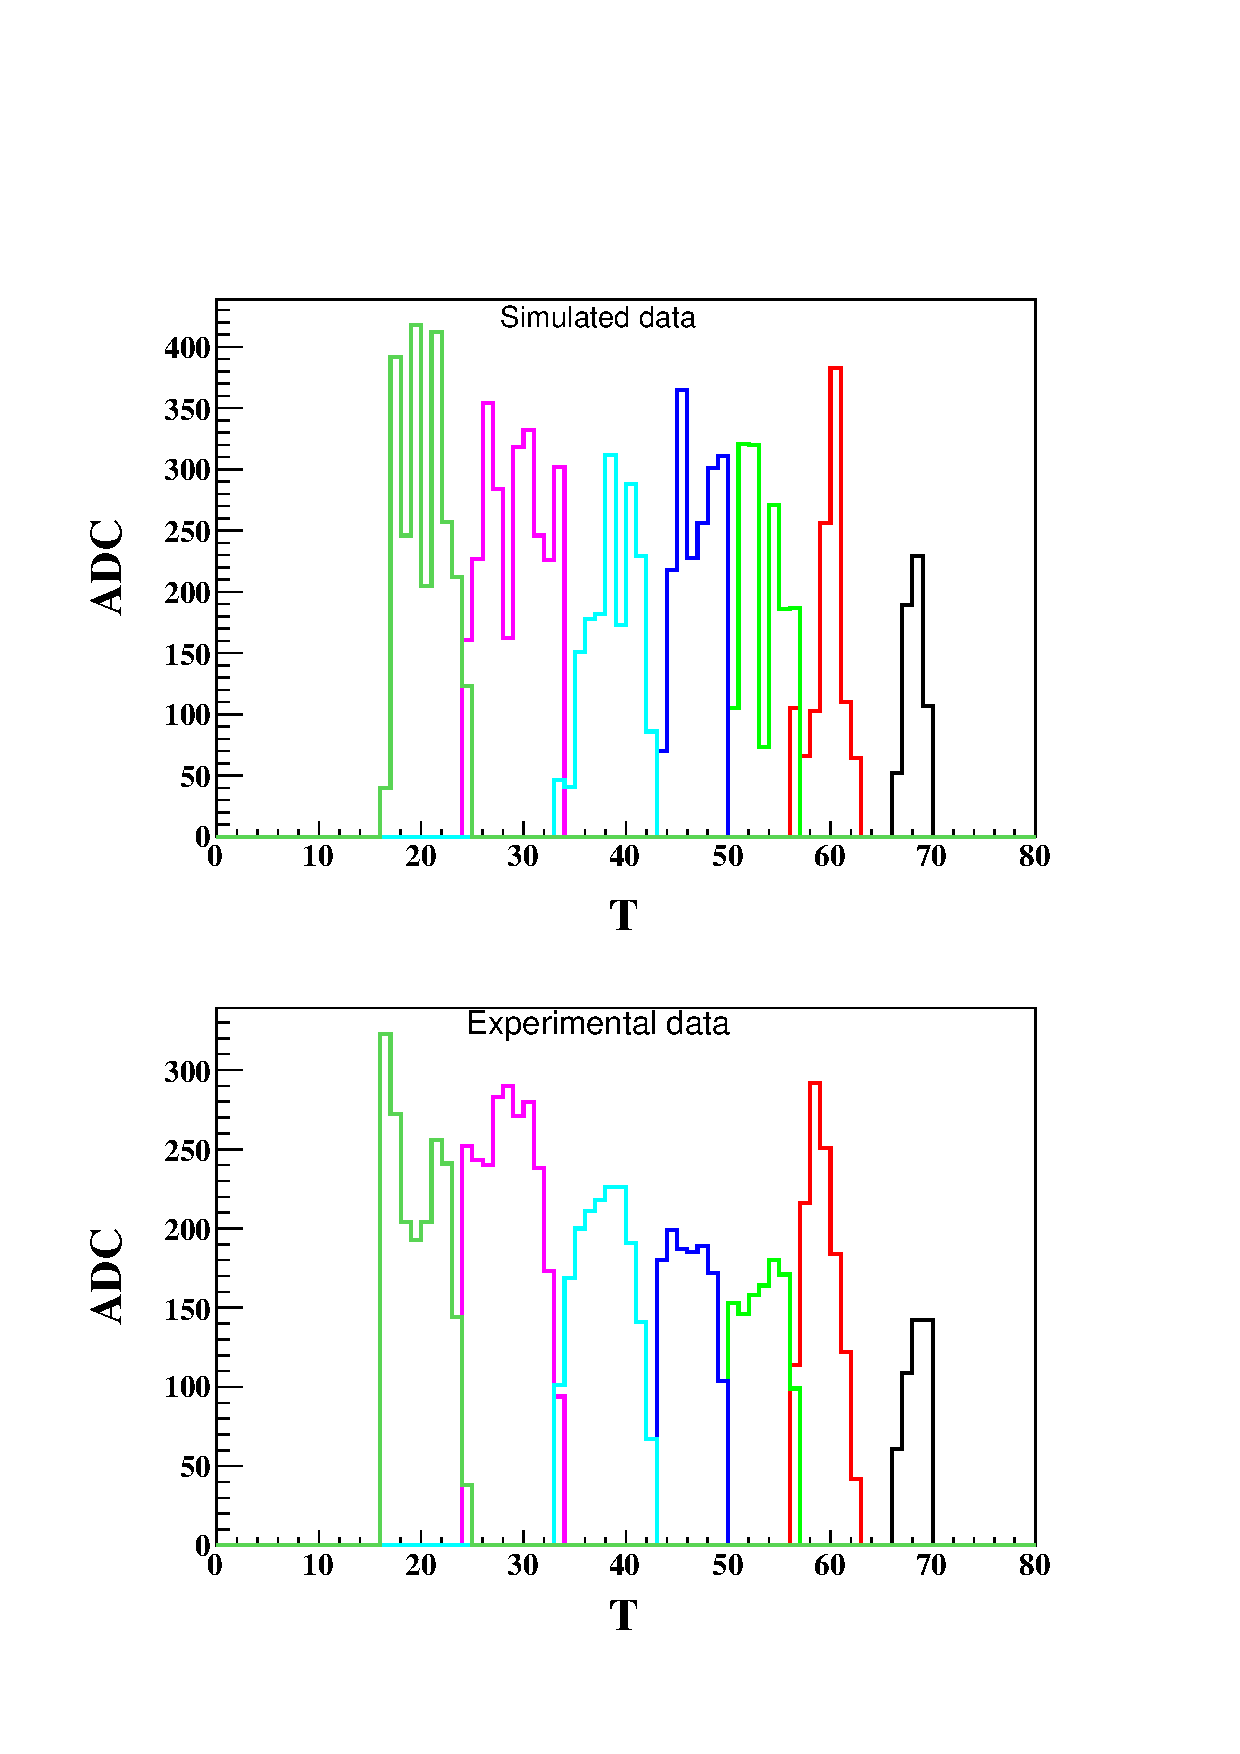
\includegraphics[scale=0.42]{fig_2017/Event_ADC_Graph_8799283.pdf}
\caption{Simulated (upper) and experimental (lower) ADC and T distributions 
of a track. The colors indicate the pads, same color in top and bottom indicate 
that they are the same pad.}
\label{fig:EVENT_adc_tdc}
\end{figure}

\begin{figure*}[tb]
\centering
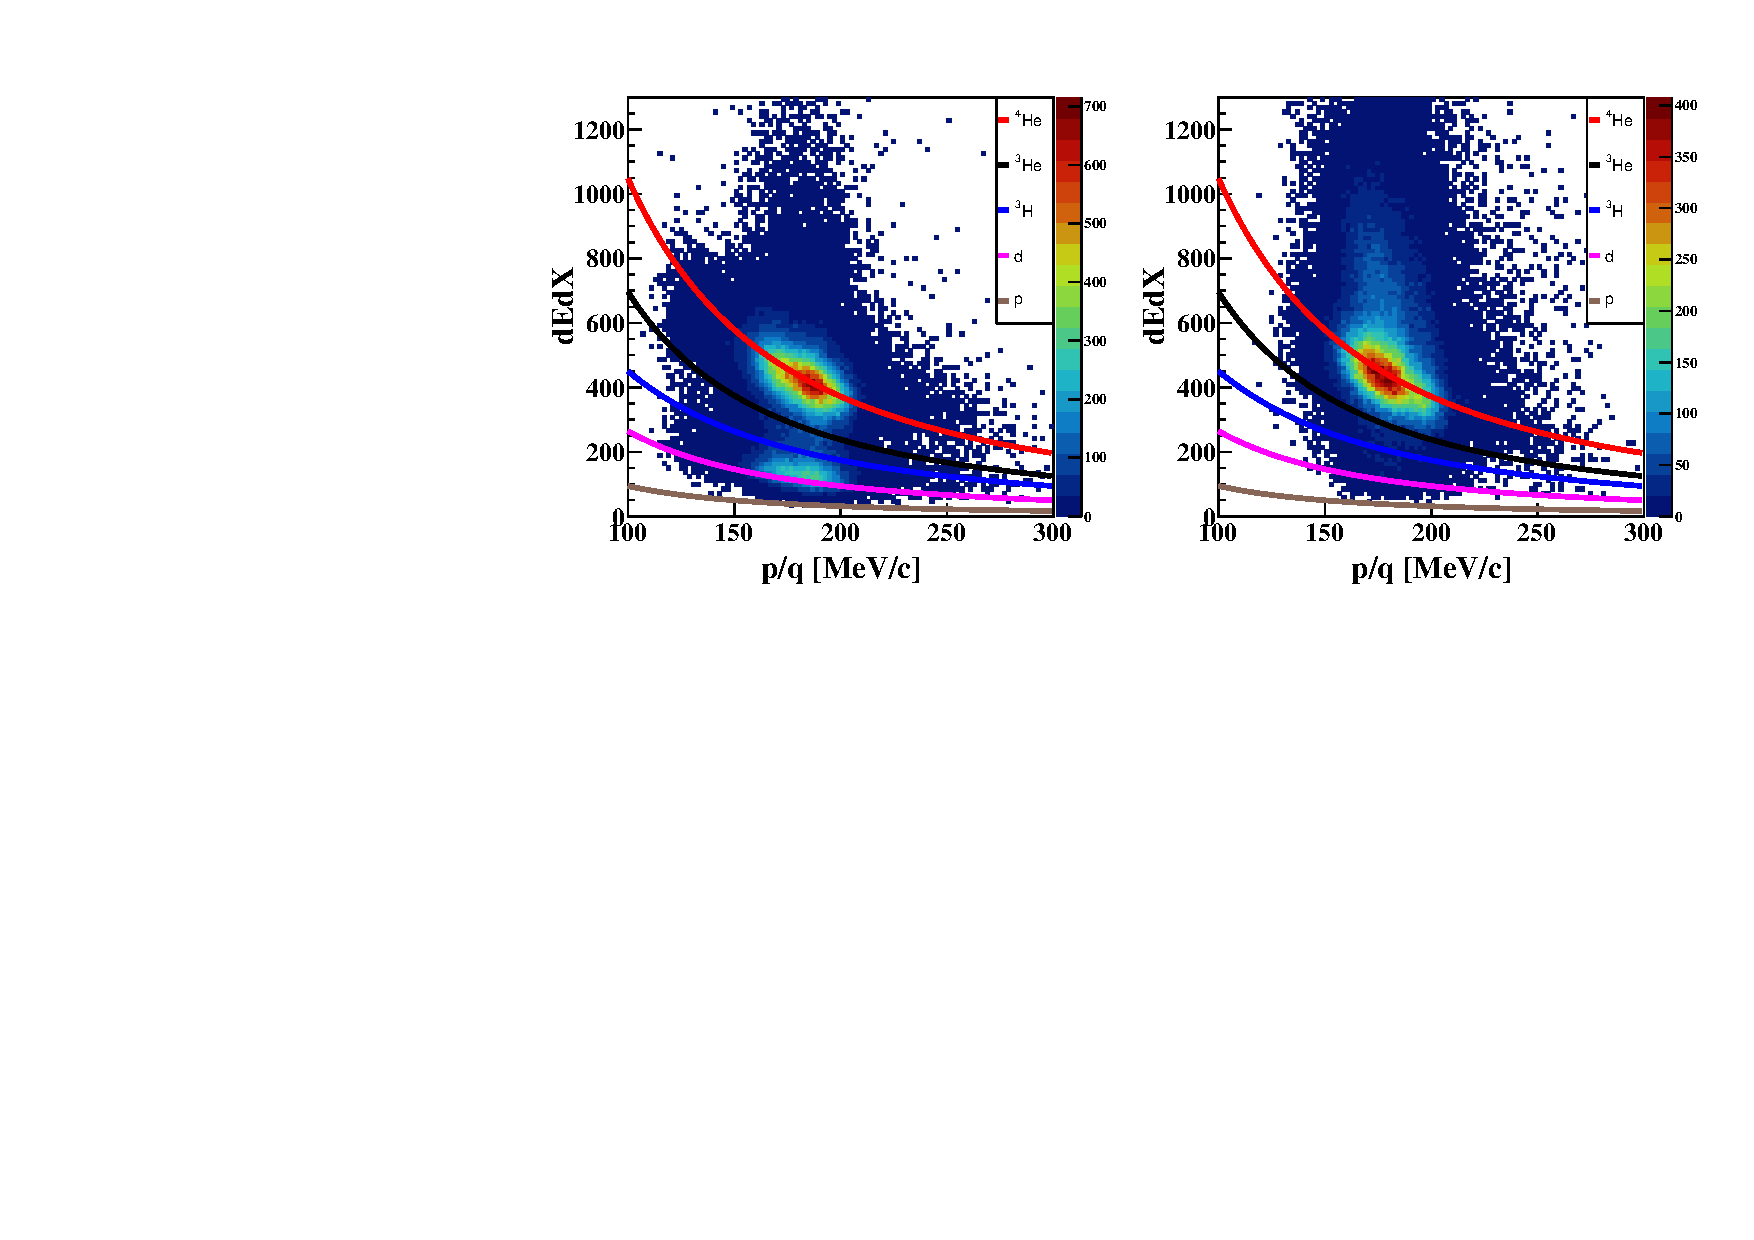
\includegraphics[scale=0.73]{fig_2017/f_dedx_p_exp_2nd.pdf}
\caption{$\small{\frac{dE}{dX}}$ vs. $p/q$ distribution for the left half of 
   the RTPC (left) and for the right half (right) after gain calibration.  
   The lines are theoretical expectations from Bethe-Bloch formula for $^4$He 
   (red), $^3$He (black), $^3$H (blue), $^2$H (pink) and protons (grey).}
\label{fig:dedx_p_exp_2nd}
\end{figure*}

\section{Track Reconstruction}
\label{sec_tracking}

\subsection{Noise Rejection}
Two independent noise signatures were identified in the raw data and removed 
in software prior to track reconstruction. Both are transient and isolated to 
a subset of the readout channels. 

The first is an oscillatory noise located early in the readout time window, 
shown in the top panel of Fig.~\ref{fig:noise} for a particularly noisy 
channel. Its amplitude is similar to those of real tracks. About 
18\% of the readout channels exhibit large contributions from this noise 
characteristic. Due to its unique time-energy correlation for the given 
channels, the noise could be removed on an event by event and channel by 
channel basis without significant loss of good signals. The result of the
procedure is illustrated in the bottom panel of Fig.~\ref{fig:noise}.

The second noise signature was a coherent noise affecting about 25\% of the 
amplifiers boards, when simultaneous hits in most of the 16 channels of the
board were recorded. An event-based technique to identify and remove this noise was developed based 
on counting simultaneous hits in each pre-amplifier group, and, if sufficiently large, 
perform a dynamic pedestal subtraction based on the average ADC of neighboring 
channels within this group.

The sources of these effects were not determined, but rejection techniques 
allowed to reconstruct 10\% more good tracks and 
recover 70 channels that were previously ignored due to excessive noise levels.

\begin{figure}[tb!]\centering
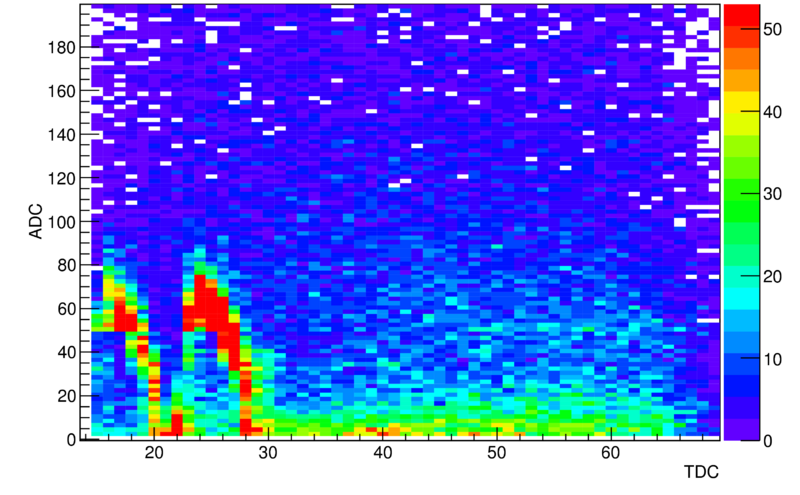
\includegraphics[scale=0.25]{fig/noisy_pad_before_rejection2.png}
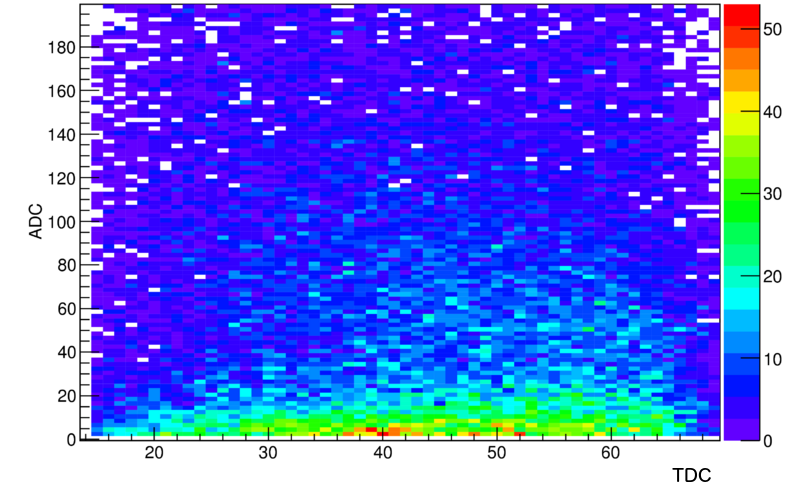
\includegraphics[scale=0.25]{fig/noisy_pad_after_rejection2.png}
\caption{The ADC vs. T spectrum for an example noisy channel before (top) and 
after (bottom) noise rejection algorithms.  Only hits associated with tracks 
are included, and the selection of events and tracks is the same in both 
plots.}
\label{fig:noise}
\end{figure}


\subsection{Track Fitting}\label{sec_rec}
We start with reconstructing the spacial origin of the hits using the extracted drift speed and drift path 
parameters. For each registered hit, we calculate a position of emission from 
the recorded time and the position of the recording pad. The third step 
is to create chains of hits. The maximum distance between two close adjacent 
hits has to be less than 10.5 mm to chain them, which roughly corresponds to 
neighbors and next to neighbors. Then, we fit the chains with a helix if they have a minimum of 
10 hits. We then eliminate from the chain the hits that are 5 mm or farther from the fit
as they are not likely part of the same track.
This new reduced chain is used for a second and final helix fit.

For energy deposition, the mean $\frac{dE}{dx}$ is calculated as
\begin{equation}
 \left\langle \frac{dE}{dX} \right\rangle= \frac{\sum\limits_{i} \frac{ADC_{i}}{G_i}}{L},
\end{equation}
where the sum runs over all the hits of the track, $G_{i}$ is the gain of 
the associated pad, and $L$ is the visible track length in the active drift 
volume. 

\section{Performance Studies}\label{sec_perfor}

The primary data sample used for calibration and performance assessment of the
RTPC was elastic scattering with a 1.2 GeV electron beam.  The electron's momentum
and direction is measured with CLAS, which uniquely determines the expected recoiling
$^4$He kinematics.  Matching requirements between reconstructed and expected $z$-vertex
and direction of the RTPC track provides a clean selection of elastically-scattered
$^4$He, shown in Fig.~\ref{fig:w}.


\begin{figure}[tb]\centering
  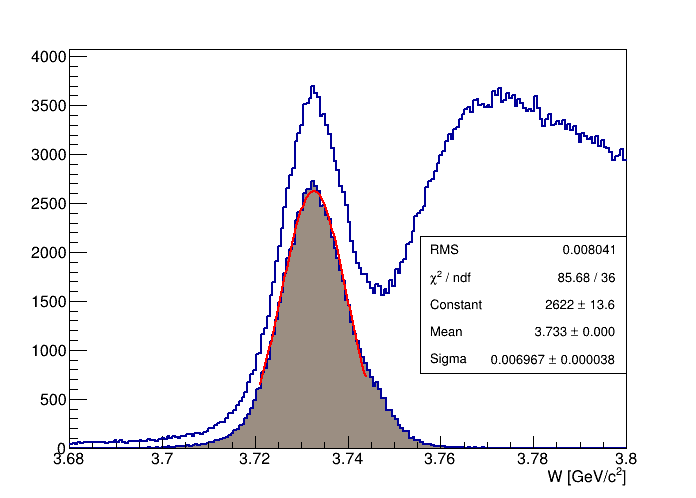
\includegraphics[width=8cm]{fig/fit_W_distribution_l.png}
  \caption{The $W$ distribution calculated from electron kinematics before (``inclusive'')
  and after (``exclusive'') requiring a matching track in the RTPC.\label{fig:w}}
\end{figure}


\subsection{Resolution}
Elastic scattering was used to estimate the tracking resolution of the RTPC 
based on the residual between the expected and measured $^4$He tracks.  The RTPC
resolutions, after removing contributions from the electron, are shown in Table
~\ref{tab:reso}, and are very similar for the two halves of the RTPC.  Note, the
$\theta$- and $z$-resolutions are highly correlated.
\begin{table}[htbp]
\begin{center}
\begin{tabular}{|l|cccc|}
  \hline
& $\sigma_{z}$ &  $\sigma_{\theta}$ & $\sigma_{\phi}$ & $\sigma_{p}$\\
\hline
Left &  5.3 mm & 3.8$^{\circ}$ & 1.9$^{\circ}$ & 9$\%$ \\
Right & 6.5 mm & 4.0$^{\circ}$ & 1.9$^{\circ}$ & 8$\%$\\
\hline
\end{tabular}
\caption{The resolutions of the two modules of the RTPC for $z$-vertex, polar and azimuthal angles, and momentum.}
\label{tab:reso}
\end{center}
\end{table}


\subsection{Efficiency}
We measured the efficiency of the RTPC
using elastic scattering on $^4$He by comparing the inclusive yield, based
only on electron detection, to the exclusive elastic yield, where the Helium
recoil is also detected (see Fig.~\ref{fig:w}). We present in Fig.~\ref{fig:rtpc_eff}
the results for the two halves of the detector. We observe that the left and 
the right modules have similar efficiencies except near the upstream target 
window. This difference is due to the large number of dead channels concentrated
in this part of the left half of the detector

\begin{figure}[tb]
\centering
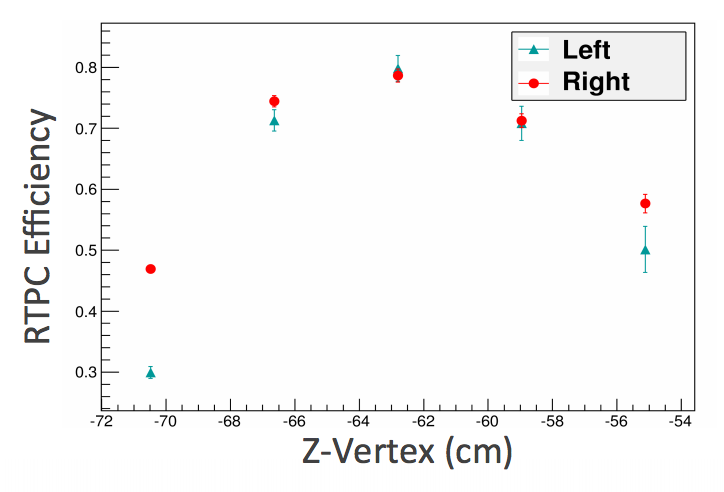
\includegraphics[width=8cm]{fig/tpceff.png}
\caption{The RTPC $^4$He detection efficiency as a function of the longitudinal 
   position along the detector.
 \label{fig:rtpc_eff}}
 \end{figure}


 \section{Conclusion}

We reported on the construction, operation and calibration of a small RTPC 
designed to measure helium-4 nuclei in high rate environment. The operation
of the detector was successful and allowed to detect helium nuclei with a 75\%
efficiency and a readout rate
of 3.1 kHz triggered by the detection of high energy electrons and 
photons in the CLAS spectrometer. 

\input acknowledgment.tex  

\begin{thebibliography}{99}

\bibitem{CLASref}
   B.A. Mecking et al., The CEBAF large acceptance spectrometer, Nucl. Inst. 
   and Meth. A 503, 513 (2003).

\bibitem{DCref}
   M.D. Mestayer et al., The CLAS drift chamber System, Nucl. Inst.  and Meth.  
   A 449, 81 (2000).

\bibitem{CCref}
   G. Adams et al., The CLAS Cerenkov detector, Nucl. Inst. and Meth. A 465, 
   414 (2001).

\bibitem{TOFref}
   E.S. Smith et al., The time-of-flight system for CLAS, Nucl.  Inst. and 
   Meth. A 432, 265 (1999).

\bibitem{ECref}
   M. Amarian et al., The CLAS forward electromagnetic calorimeter, Nucl.  
   Inst. and Meth. A 460, 239 (2001). 

\bibitem{FX}
   F.X. Girod et al. (CLAS Collaboration), Measurement of Deeply virtual Compton 
   scattering beam-spin asymmetries, Phys.Rev.Lett. 100 (2008) 162002

\bibitem{Hyon-suk}
   Hyon-Suk Jo, Etude de la Diffusion Compton Profond{\'e}ment Virtuelle Sur le 
   Nucl{\'e}on avec le D{\'e}tecteur CLAS de Jefferson Lab: Mesure des Sections 
   Efficaces polaris{\'e}es et non polaris{\'e}es, IPNO-Thesis, 2007.

\bibitem{proposal1}
   G Asryan et al., Meson spectroscopy in the Coherent Production on $^{4}$He with CLAS, Jlab 
   proposal to PAC31 (2007).

\bibitem{proposal2}
   K. Hafidi et al., Deeply virtual Comton scattering off $^{4}$He, Jlab 
   proposal to PAC33 (2008).

\bibitem{BONUS-NIM}
   Howard C. Fenker et al., BoNuS: Development and Use of a Radial TPC using 
   Cylindrical GEMs, Nucl. Instrum. Meth. A592, 273-286 (2008)

\bibitem{GEM_ref_pic}
   F. Sauli, The Gas Electron Multiplier (GEM): Operating Principles and 
   Applications, Nucl. Instr. and Meth, A805(2016)2

\bibitem{GEM_ref}
   J. Beringer et al. (Particle Data Group), Particle detectors at 
   accelerators, Phys. Rev. D 86, 010001, pages: 339-368, 2012.

\bibitem{MAGBOLTZ}
   S. Biagi, Monte Carlo simulation of electron drift and diffusion in counting 
   gases under the influence of electric and magnetic fields, Nucl.  Inst. and 
   Meth. in Phy. Res. A, vol. 421, pp. 234-240, 1999.

 \bibitem{ALICE-FEE}
 L. Musa et al., The ALICE TPC front end electronics, 2003 IEEE Nuclear 
 Science Symposium, 2003, pp. 3647-3651 Vol.5
 
 \bibitem{ALICE-PASA}
   H.~K.~Soltveit {\it et al.},
   ``The Preamplifier shaper for the ALICE TPC-Detector,''
   Nucl.\ Instrum.\ Meth.\ A {\bf 676} (2012) 106
 
 \bibitem{ALICE-ALTRO},
 R. E. Bosch, {\it et al.}, ``The ALTRO chip: a 16-channel A/D converter and 
 digital processor for gas detectors'', IEEE Transactions on Nuclear Science, 
 vol. 50, no. 6, pp. 2460-2469, Dec. 2003.

\bibitem{GEANT4}
http://geant4.cern.ch
 	

\end{thebibliography}

\end{document}

